% kompilowac pdflatex-em
\documentclass[a4paper,11pt]{article}
\usepackage[T1]{fontenc}
\usepackage[utf8]{inputenc}	% konwersja plików wejściowych LaTeXa
\usepackage[polish, english]{babel}
\usepackage{polski}
\usepackage{lmodern}		% Latin Modern — cleaner T1 CM variant
\usepackage{graphicx}		% wstawianie, manipulowanie grafika
\usepackage{geometry}		% do ustawienia marginesow
\usepackage{url}		% obsluga url
\usepackage{hyperref}		% odnosniki (tabele, bibliografia,itp.) będą linkami,
\usepackage{multirow}
\usepackage{color}


% marginesy {lewy,,prawy}
\geometry{hdivide={1.45cm,,1.45cm}}
% marginesy {gora,,dol}
\geometry{vdivide={1.6cm,,1.6cm}}

% ustawienie odstępów między wierszami na 1.5
\renewcommand\baselinestretch{1.2}

% \hline\hline da linię Lesz
\setlength{\doublerulesep}{\arrayrulewidth}

\pagestyle{empty}


\hypersetup{
  pdftitle={Rafal Leszko - curriculum vitae},
  pdfauthor={Rafal Leszko},
  %pdfstartview={FitBH},
}

\makeatletter
\def\section{\@ifstar\unnumberedsection\numberedsection}
\def\numberedsection{\@ifnextchar[%]
  \numberedsectionwithtwoarguments\numberedsectionwithoneargument}
\def\unnumberedsection{\@ifnextchar[%]
  \unnumberedsectionwithtwoarguments\unnumberedsectionwithoneargument}
\def\numberedsectionwithoneargument#1{\numberedsectionwithtwoarguments[#1]{#1}}
\def\unnumberedsectionwithoneargument#1{\unnumberedsectionwithtwoarguments[#1]{#1}}
\def\numberedsectionwithtwoarguments[#1]#2{%
  \ifhmode\par\fi
  \removelastskip
  \vskip 5ex\goodbreak
  \refstepcounter{section}%
  \hbox to \hsize{\hss\vbox{\advance\hsize by 0cm
      \noindent
      \leavevmode\Large\bfseries\raggedright
      \thesection.\ 
      #2\par
      \vskip -2.2ex
      \noindent
      \textcolor[rgb]{0.5,0.5,0.5}{\rule{\textwidth}{0.5pt}}
      }}\nobreak
  \vskip 2ex\nobreak
  \addcontentsline{toc}{section}{%
    \protect\numberline{\thesection}%
    #1}%
  }
\def\unnumberedsectionwithtwoarguments[#1]#2{%
  \ifhmode\par\fi
  \removelastskip
  \vskip 5ex\goodbreak
%  \refstepcounter{section}%
  \hbox to \hsize{\hss\vbox{\advance\hsize by 0cm
      \noindent
      \leavevmode\Large\bfseries\raggedright\sc
%      \thesection\
      #2\par
      \vskip -2.2ex
      \noindent
%\hrulefill
\textcolor[rgb]{0.5,0.5,0.5}{\rule{\textwidth}{0.5pt}}
      }}\nobreak
  \vskip 2ex\nobreak
  \addcontentsline{toc}{section}{%
%    \protect\numberline{\thesection}%
    #1}%
  }
  


\makeatother
\pagestyle{empty}

\newcommand{\poz}[2]{
\noindent{#2 \hfill \textsc{#1}}\\
}

\setlength\parindent{0pt}

\newcommand{\cvsection}[1]{\vspace{-7.5pt} \section*{#1} \vspace{-3.75pt}}

\newenvironment{changemargin}[2]{%
\begin{list}{}{%
\setlength{\topsep}{0pt}%
\setlength{\leftmargin}{#1}%
\setlength{\rightmargin}{#2}%
\setlength{\listparindent}{\parindent}%
\setlength{\itemindent}{\parindent}%
\setlength{\parsep}{\parskip}%
}%
\item[]}{\end{list}}
	
\newenvironment{text}{
\setlength\parindent{0pt}
	\vspace{-7.5pt}
	\begin{changemargin}{6pt}{0cm}

		\renewcommand\baselinestretch{1.03}
		\noindent
		\hspace{-2.25pt}}
		{\end{changemargin}\vspace{3.75pt}}

\newenvironment{cvtabular}%
{%
	}%
	{}%

\newenvironment{cvheader}%
		{\begin{changemargin}{1.5pt}{0cm} \begin{tabular}{p{0.28\textwidth} p{0.44\textwidth} p{0.33\textwidth}}%
	%
	}
	{\end{tabular}\end{changemargin}}%

	\newcommand{\bul}[1]{\mbox{$\bullet$ #1 \vspace{2.25pt}}}


\begin{document}

	{\renewcommand{\arraystretch}{1.1}
	\begin{cvheader}
		\multicolumn{2}{l}{} & \multirow{5}{*}{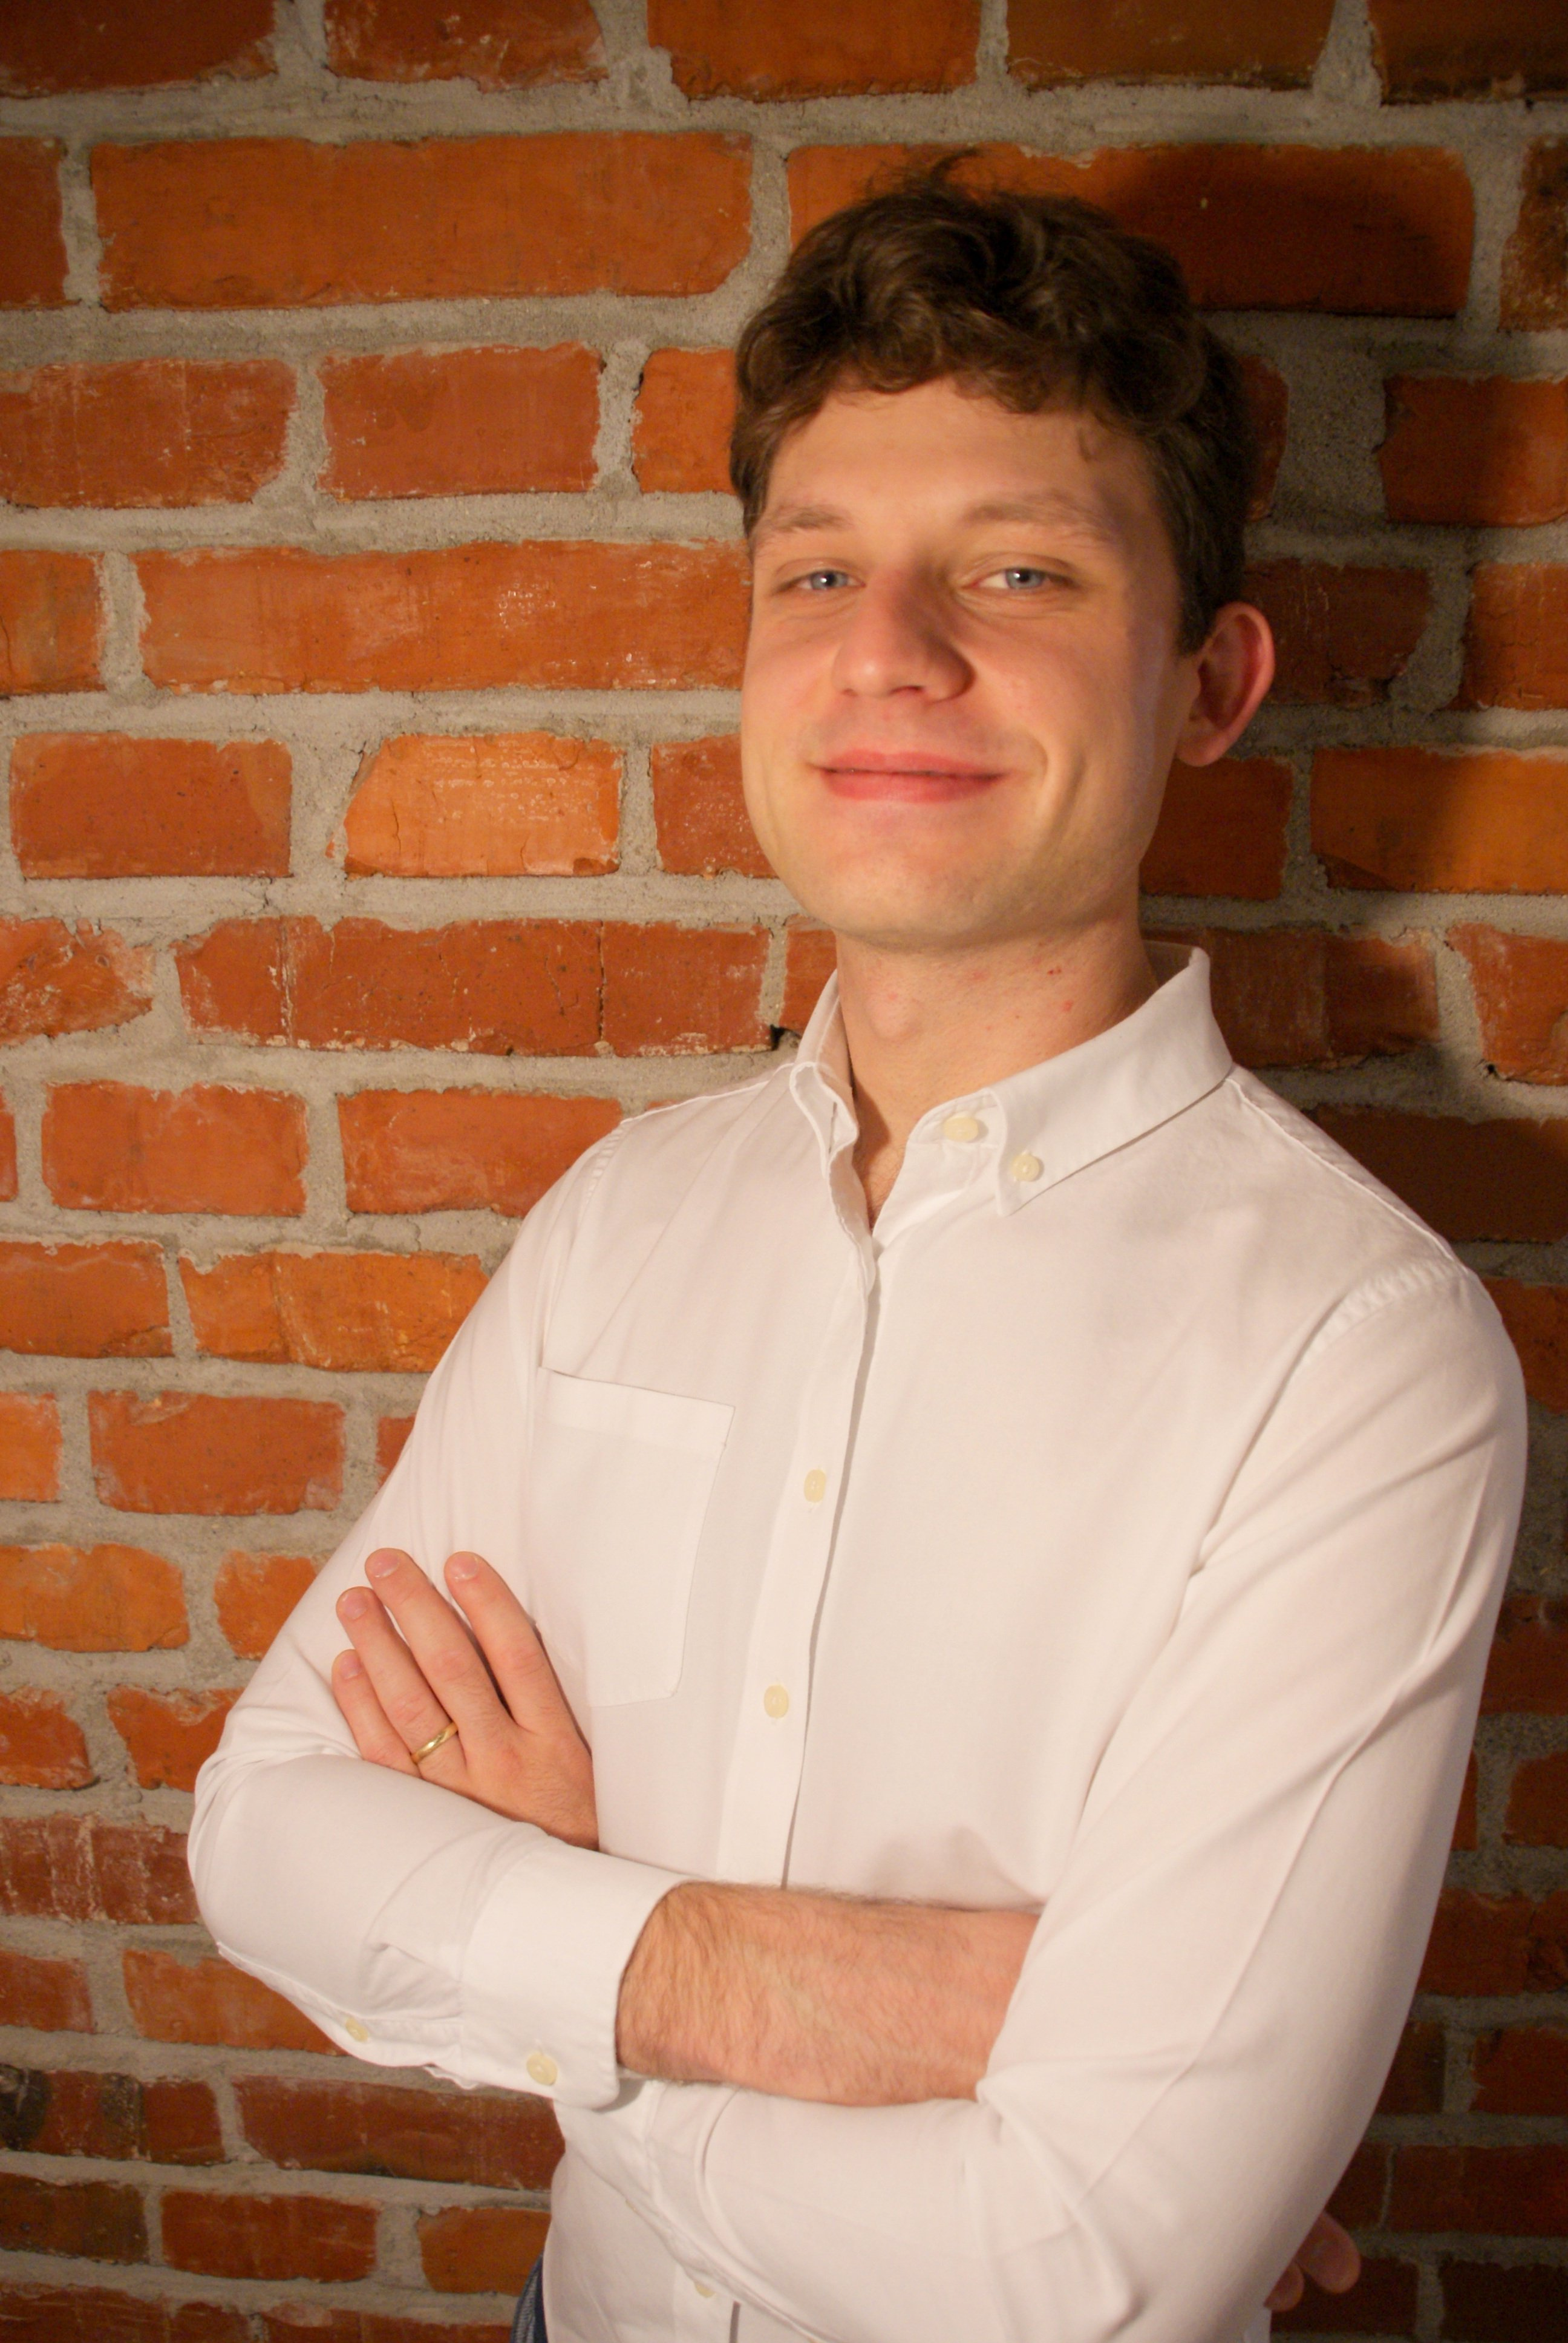
\includegraphics[width=3.6cm]{photo.jpg}}\\[-4.5pt]
		\multicolumn{2}{l}{\large{\textsc{\textbf{Rafał Leszko, M.Sc.}}}} & \\[2.25pt]
		\multicolumn{2}{l}{\large{\textsc{\textbf{Lead AI Engineer (Real-time Generative AI)}}}} & \\[-3.75pt]
		\textsc{} &   & \\
		\textsc{website} & \href{https://www.rafalleszko.com/}{rafalleszko.com} & \\
		\textsc{email} & rafal.leszko@gmail.com & \\
		\textsc{location} & Krakow, Poland & \\[0.1cm]
	\end{cvheader}}
	
\cvsection{personal statement}

I am a \textbf{Lead AI Engineer} at Daydream/Livepeer and the \textbf{lead developer} on \underline{\href{https://github.com/daydreamlive/scope}{Scope}} - a \textbf{real-time} engine for \textbf{interactive audio/video AI generation}, running pipelines like video diffusion, LTX-2 and ACEStep on \textbf{NVIDIA RTX 4090/5090} (and H100/H200).

I work across the stack on real-time generative AI systems: \textbf{architecture}, \textbf{rapid prototyping}, and \textbf{high- and low-level development}. I code daily in \textbf{Python} and \textbf{Go}, with prior experience at \textbf{Hazelcast}, \textbf{Google}, and \textbf{CERN}. I have spoken at \textbf{70+ conferences} (including \textbf{KubeCon} twice) and authored \textbf{a book}.\\[-3.75pt]

\cvsection{professional experience}

\begin{cvtabular}
	\poz{Nov 2021 -- present}{\textbf{Livepeer / Daydream, Remote}}
	\poz{}{\textbf{Go/Blockchain Engineer → Staff Engineer → Lead AI Engineer}}
	\end{cvtabular}

	\begin{text}
	As lead developer on \underline{\href{https://github.com/daydreamlive/scope}{Scope}}, I own architecture, integrate new model research, and drive end-to-end performance.
	% TODO: replace with concrete numbers - e.g. "Drove X FPS at Y ms p99 on H100", "Cut TTFT by N\%", "Reduced inference cost to \$Z/min".
	Earlier at Livepeer I shipped core video infrastructure across \underline{\href{https://github.com/livepeer/go-livepeer}{Livepeer Node}}, \underline{\href{https://github.com/livepeer/catalyst}{Decentralized Media Server}}, and \underline{\href{https://github.com/livepeer/studio}{Livepeer Studio}}. \\[0.1cm]
	\bul{Python} \bul{PyTorch} \bul{CUDA} \bul{Diffusion Models} \bul{Video/Audio Generation} \bul{WebRTC} \bul{Go} \\[-0.3cm]
	\end{text}

\begin{cvtabular}
\poz{Mar 2018 -- Sep 2021}{\textbf{Hazelcast, Remote}}
\poz{}{\textbf{Cloud Software Engineer → Cloud-Native Tech Lead}}
\end{cvtabular}

\begin{text}
I built Hazelcast's cloud integrations: the \textbf{Kubernetes Operator}, \textbf{Helm Chart}, \textbf{plugins} (Kubernetes, AWS, GCP, Azure, Zookeeper), and \textbf{Docker images}. \\[0.1cm]
\bul{Go} \bul{Kubernetes} \bul{Java} \bul{Helm} \bul{AWS} \bul{Azure} \bul{GCP} \bul{Docker} \\[-0.3cm]
\end{text}

\begin{cvtabular}
\poz{Sep 2016 -- Feb 2018}{\textbf{Google, Krakow}}
\poz{}{\textbf{Senior Software Engineer}}
\end{cvtabular}

\begin{text}
I designed and built a microservice-based project-tracking system. \\[0.1cm]
\bul{Spanner} \bul{GCP} \bul{Java} \bul{Pub/Sub} \bul{Microservices} \bul{CI/CD} \\[-0.3cm]
\end{text}

\begin{cvtabular}
\poz{Oct 2015 -- Jul 2016}{\textbf{Zooplus, Krakow, Lead Engineer}}
\end{cvtabular}

\begin{text}
\bul{Java}  \bul{Spring Boot} \bul{Hibernate} \bul{Oracle} \bul{MongoDB} \bul{Mesos} \bul{CI/CD} \\[-0.3cm]
\end{text}

\begin{cvtabular}
\poz{Dec 2013 -- Sep 2015}{\textbf{Luxoft for UBS, Krakow, Tech Lead}}
\end{cvtabular}

\begin{text}
\bul{Big data} \bul{Java} \bul{Oracle PL/SQL} \bul{Fitnesse} \\[-0.3cm]
\end{text}

\begin{cvtabular}
		\poz{Oct 2010 -- May 2013}{\textbf{AGH University, Krakow, Java Developer}}
			\end{cvtabular}
\begin{text}
\bul{Distributed computing} \bul{Eclipse RCP} \bul{OSGi} \bul{Java} \bul{Web Services} \\[-0.3cm]
\end{text}

\begin{cvtabular}
		\poz{Jul 2009 -- Sep 2009, Mar 2011 -- Apr 2012}{\textbf{CERN, Geneva, Software Engineer}}
	\end{cvtabular}
	\begin{text}
\bul{LHC Data Visualization} \bul{Java} \bul{Spring} \bul{C++} \bul{Oracle} \bul{SQL} \\[-0.3cm]
\end{text}

\cvsection{education}
	\begin{cvtabular}
		\poz{2012 -- 2014}{\textbf{PhD candidate in Computer Science}, AGH University of Science and Technology}
			\end{cvtabular}\\[-3.75pt]
	\begin{cvtabular}
		\poz{2006 -- 2012}{\textbf{M.Sc. in Computer Science}, AGH University of Science and Technology}
			\end{cvtabular}

\cvsection{other achievements}

\begin{cvtabular}
		\poz{Apr 2016 -- present}{\textbf{I presented at \underline{\href{https://www.rafalleszko.com/talks}{70+ software conferences}}} (including KubeCon twice)}
			\end{cvtabular}\\[-15pt]

	\begin{cvtabular}
		\poz{Aug 2017}{\textbf{I authored a book} \underline{\href{https://www.packtpub.com/product/continuous-delivery-with-docker-and-jenkins-second-edition/9781838552183}{"Continuous Delivery with Docker and Jenkins"}}}
			\end{cvtabular}\\[-15pt]

	\begin{cvtabular}
		\poz{Dec 2015 -- present}{\textbf{I write \underline{\href{https://www.rafalleszko.com/blog}{blog posts}}} (including for OpenShift)}
			\end{cvtabular}\\[-15pt]

	\begin{cvtabular}
		\poz{Apr 2014}{\textbf{I wrote a scientific paper} \underline{\href{https://core.ac.uk/display/236278467}{"Verification Mechanism For Lightweight Component-based}}\\ \underline{\href{https://core.ac.uk/display/236278467}{Environment Based On IoC Container"}}}
			\end{cvtabular}\\[-15pt]



\cvsection{interests}

On a more personal note, I love \textbf{running ultramarathons} and \textbf{mountaineering}. During my time at CERN, I was also an official \textbf{CERN guide}, explaining physics and CERN to visitors. For years I was a \textbf{coordinator}, \textbf{team leader}, and \textbf{trainer} in the \textbf{Szlachetna Paczka} charity.\\[-3.75pt]

\end{document}
